\documentclass{beamer}
\usepackage{graphicx}
\usepackage{tikz}
\usetikzlibrary{shapes,arrows}
\usepackage{tikz}
%\usecolortheme{seahorse}
  \setbeamertemplate{footline}[page number]
\usepackage{multirow}
\setbeamertemplate{navigation symbols}{}
\setbeamertemplate{frametitle}[default][center]
\setbeamerfont{frametitle}{shape=\scshape}
\usepackage{color}

\usepackage{csquotes}

\usepackage{xcolor}

\usepackage[flushleft]{threeparttable}

{\title{\textsc{Econ 352 - Money, Banking, Price, and Monetary Policy} \\ \tiny (See Williamson Ch. 12)}
\author{Trevor S. Gallen}
\date{}
\begin{document}
\renewcommand*{\inserttotalframenumber}{\pageref{lastframe}}


\setbeamertemplate{caption}{\raggedright\insertcaption\par}

\begin{frame}
\titlepage
\end{frame}

\begin{frame}
\frametitle[alignment=center]{Introduction}
\begin{itemize}
\item Thus far our model is ``real"--no money
\bigskip
\item But money helps overcome frictions and itself may open the door to new frictions
\bigskip
\item So let's try to put in money
\bigskip
\item Most important relationship between real and nominal worlds: the Fisher relation
\bigskip
\item But first: what is money?
\end{itemize}
\end{frame}

\begin{frame}
\frametitle[alignment=center]{What is Money?}
\begin{itemize}
\item Money has three functions:
\bigskip
\begin{enumerate}
\item Medium of exchange:  it's used to transact
\bigskip
\item Store of value: money today can be used tomorrow
\bigskip
\item Unit of account: we measure things in it
\end{enumerate}
\bigskip
\item The most important role is as a medium of exchange--stocks \& bonds are stores of value
\bigskip
\item How do we measure it?
\end{itemize}
\end{frame}

\begin{frame}
\frametitle[alignment=center]{Definitions of Money}
\begin{itemize}
\item Many measures of money
\bigskip
\begin{itemize}
\item M0, physical currency
\bigskip
\item Monetary Base: physical currency + bank deposits at Fed
\bigskip
\item M1:  M0 + demand deposits at bank
\bigskip
\item M2:  M1 + savings deposits, money market mutual funds
\end{itemize}
\bigskip
\item Let's look at MB, M1, M2
\end{itemize}
\end{frame}

\begin{frame}
\frametitle[alignment=center]{Money over time}
\begin{figure}
\centering
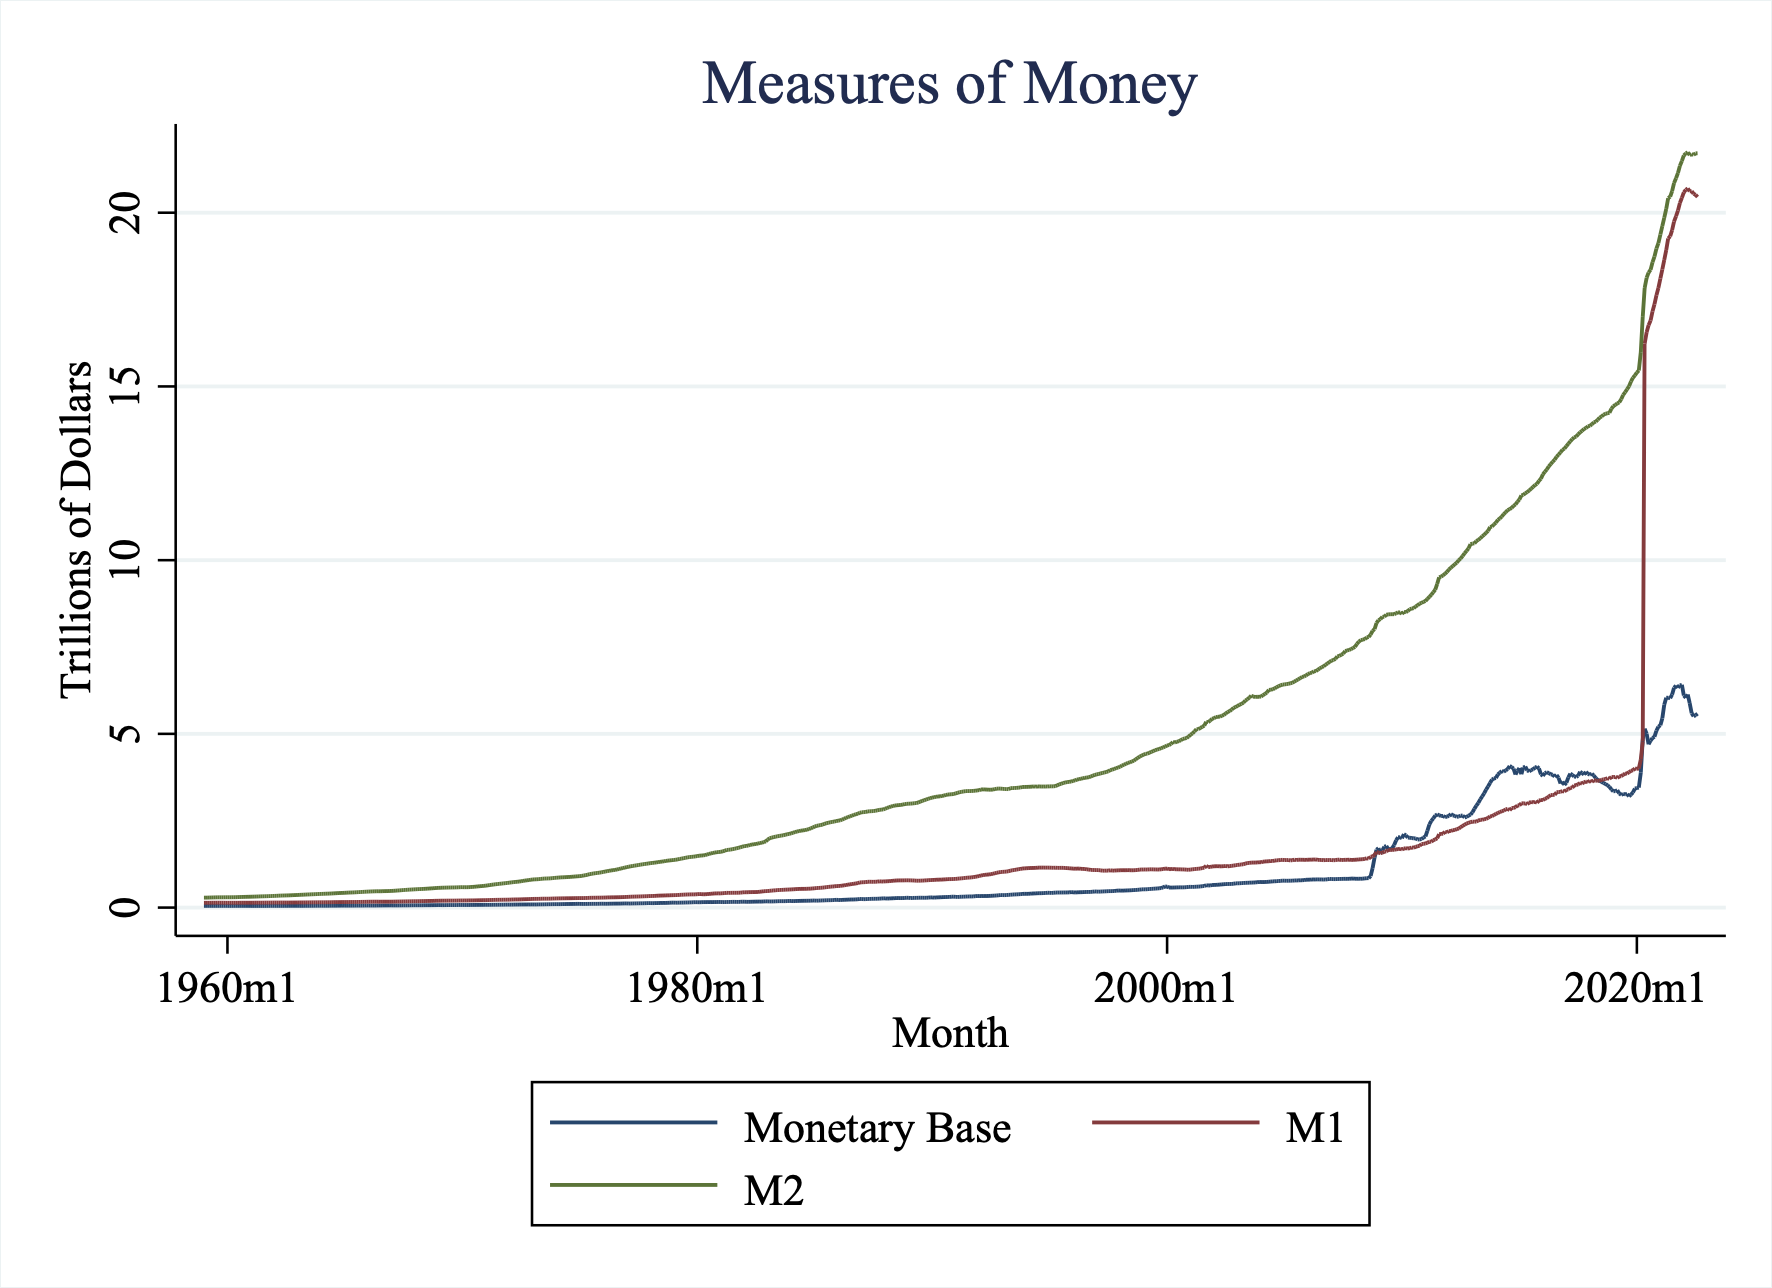
\includegraphics[scale=0.3]{Figures/MoneyoverTime.png}
\end{figure}
Monetary base was higher than physical currency \& demand deposits briefly, because bank deposits  at Fed (unrelated to demand deposits) were higher
\end{frame}

\begin{frame}
\frametitle[alignment=center]{Quantity of Money}
\begin{itemize}
\item While the amounts of money have risen precipitously, it isn't a major focus of central bankers, as we'll see
\bigskip
\item Instead, $M$ will be treated as residual of another choice, rather than something to be controlled directly
\bigskip
\item Rather than thinking about money demand directly, we'll first establish a relationship between real interest rates, nominal interest rates, and inflation, then about money demand
\end{itemize}
\end{frame}

\begin{frame}
\frametitle[alignment=center]{Fisher Relation}
\begin{itemize}
\item Now, we have dollar assets.
\smallskip
\item Call the ``real" rate of interest $r$, the ``nominal" rate of interest $R$, and the inflation rate $i$.  
\smallskip
\item Define the net inflation rate as the net change in the price level:
$$i=\frac{P'-P}{P}$$
\smallskip
\item Invest \$1 today, get back 1+$R$ dollars tomorrow.  In real terms, invest real 1/P real goods today to get (1+R)/P' tomorrow:
$$1+r=\frac{\frac{1+R}{P'}}{1/P}=\frac{1+R}{\frac{P'}{P}}=\frac{1+R}{1+i}$$
\item This is known as the Fisher relation, which we sometimes write as:
$$r=R-i$$
\item This is a definition!  Now the effect.
\end{itemize}
\end{frame}

\begin{frame}
\frametitle[alignment=center]{Fisher Effect}
\begin{itemize}
\item Fisher effect:  $\left.\frac{d R}{d i}\right|_{r=\bar{r}}=1$, nominal interest rates will follow inflation, if real rates are set by real economy/MPK 
\bigskip
\item Let's do a scatterplot with $i$ on the x-axis and $R$ on the y-axis
\bigskip
\item We'll also show the real interest rate, calculated as $r=R-i$
\end{itemize}
\end{frame}

\begin{frame}
\frametitle[alignment=center]{Fisher Effect}
\begin{figure}
\centering
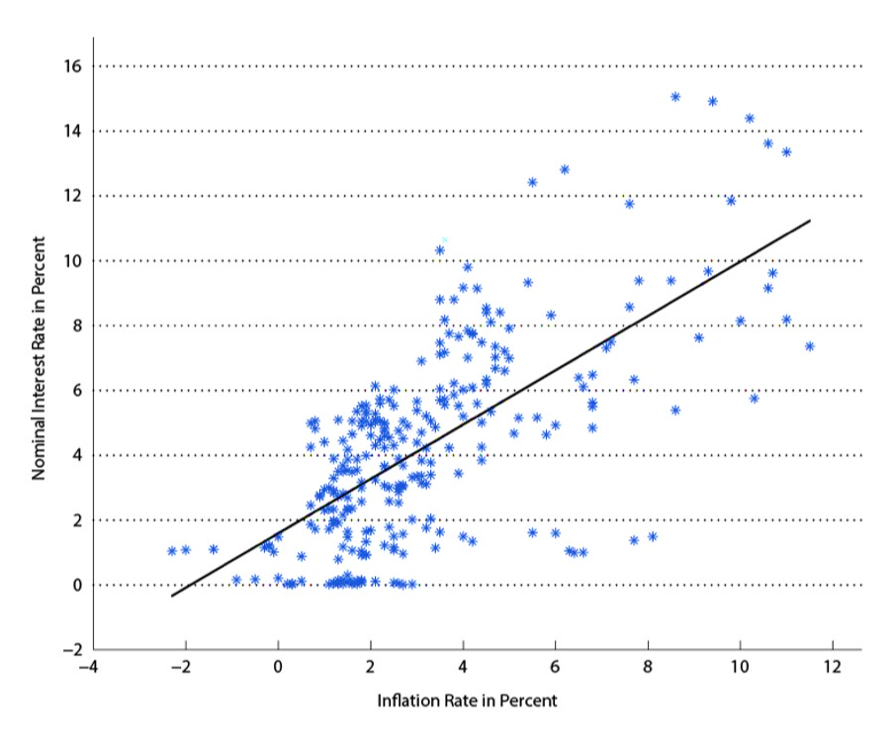
\includegraphics[scale=0.65]{Figures/W_Fig_12pt1.png}
\end{figure}
\end{frame}

\begin{frame}
\frametitle[alignment=center]{Real Interest Rate}
\begin{figure}
\centering
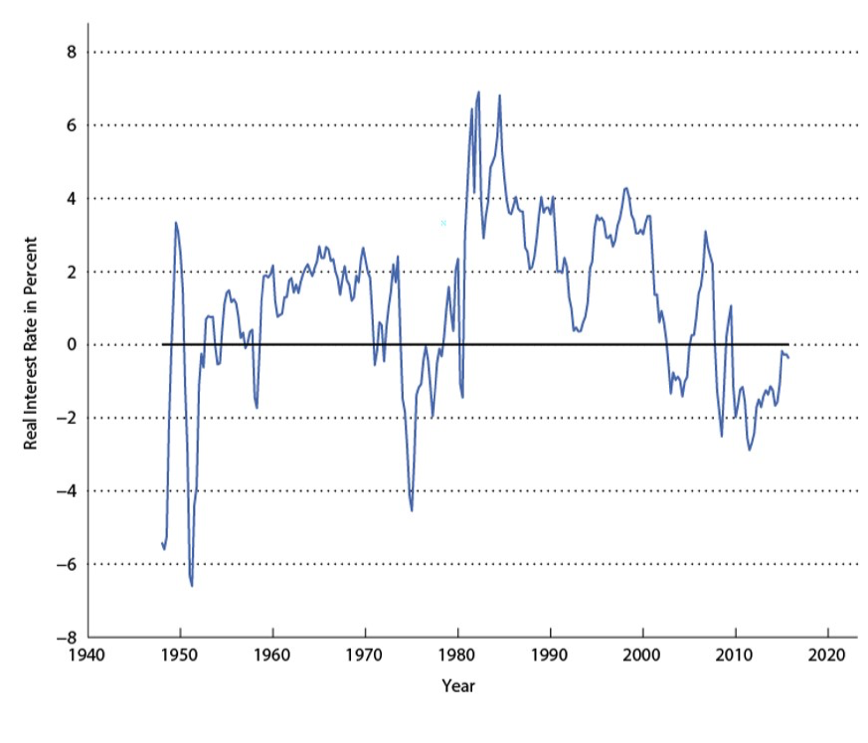
\includegraphics[scale=0.65]{Figures/W_Fig_12pt2.png}
\end{figure}
\end{frame}


\begin{frame}
\frametitle[alignment=center]{Banks and Methods of Payment}
\begin{itemize}
\item We need a market for money
\bigskip
\item But there are many definitions of money!
\bigskip
\item We'll have two big ones:  actual currency (dollars and cents) and ``other"
\bigskip
\item Other means checks (15\%), debit cards (38\%), credit cards (21\%), prepaid cards (7\%), and ACH transfers (18\%)
\bigskip
\item We'll collapse all those ``other" into ``credit cards," which just means banks acting as an intermediary to create IOUs
\bigskip
\item Credit cards cost money to operate, and so sell for some price $q$.  Credit card supply curve is thus $X^s(q)$
\end{itemize}
\end{frame}

\begin{frame}
\frametitle[alignment=center]{Credit Supply}
\begin{figure}
\centering
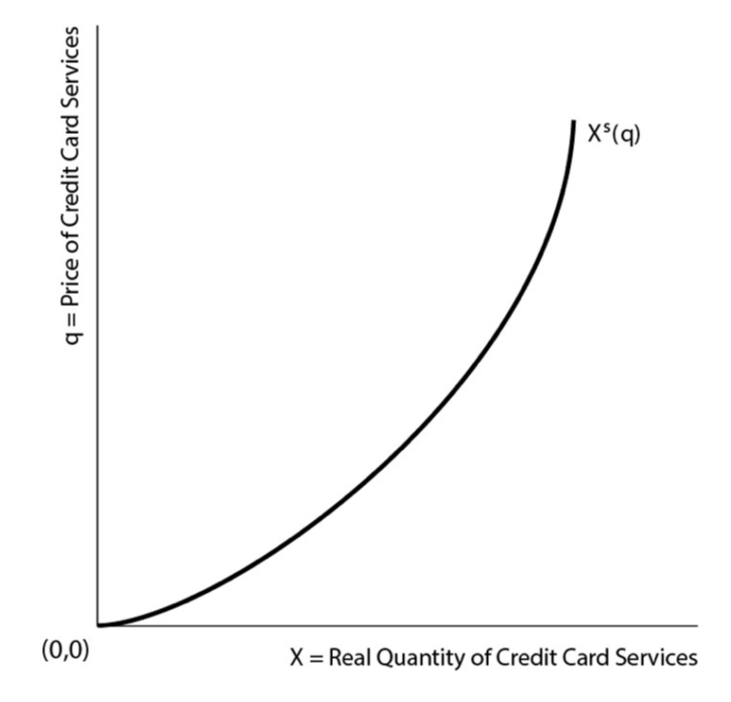
\includegraphics[scale=0.65]{Figures/W_Fig_12pt3.png}
\end{figure}
\end{frame}

\begin{frame}
\frametitle[alignment=center]{Credit Demand}
\begin{itemize}
\item Households have spending $Y$, and purchase $X^d(q)$ of it with credit cards, and $Y-X^d(q)$ in cash
\bigskip
\item What is marginal benefit, marginal cost of credit?
\bigskip
\item If purchase with credit, then over course of month make $P(1+R)$, but must pay $P(1+q)$ units to the credit card company
\bigskip
\item Can see that for households to be on interior solution (do both) need $q=R$, perfectly elastic demand
\bigskip
\item Now we have equilibrium
\end{itemize}
\end{frame}


\begin{frame}
\frametitle[alignment=center]{Credit Supply \& Demand}
\begin{figure}
\centering
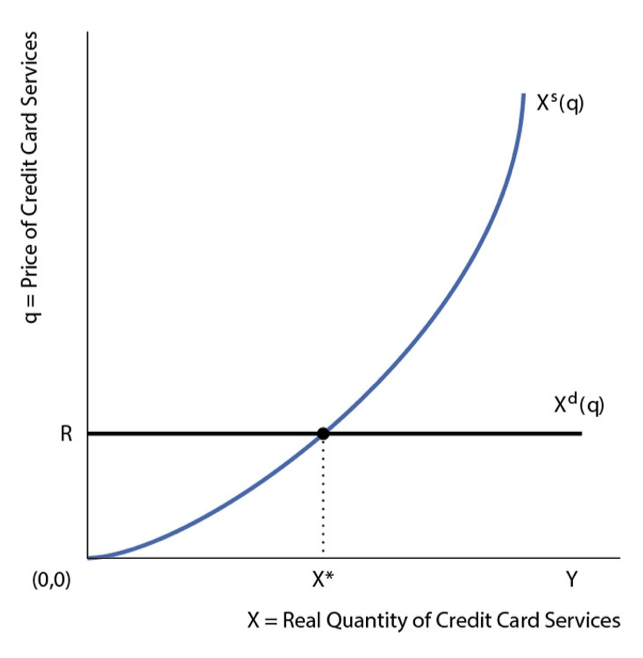
\includegraphics[scale=0.65]{Figures/W_Fig_12pt4.png}
\end{figure}
\end{frame}


\begin{frame}
\frametitle[alignment=center]{Equilibrium}
\begin{itemize}
\item What happens when nominal interest rates rise?
\bigskip
\item Benefit to using credit increases
\bigskip
\item Demand shifts up, so we shift out on the credit supply curve
\bigskip
\item And we can write money demand as the amount of dollars we need for our non-credit transactions, where $X^*$ is the equilibrium credit demand/supply:
$$M^D=P(Y-X^*(R))$$
\item Which we can instead write using the real money demand function $L$ as:
$$M^D=PL(Y,R)$$
\item Money demand is increasing in Y and decreasing in $R$
\end{itemize}

\end{frame}
\begin{frame}
\frametitle[alignment=center]{Effect of Nominal Interest Rate on Credit}
\begin{figure}
\centering
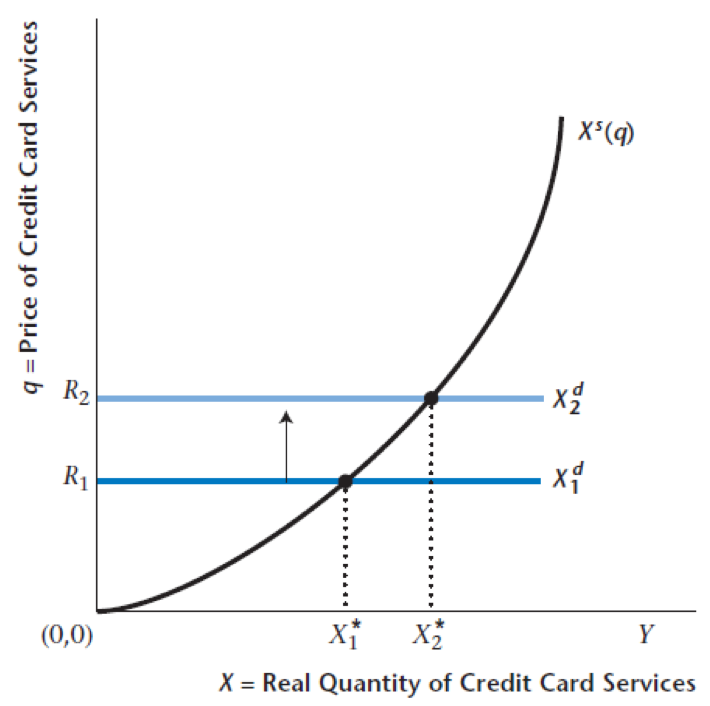
\includegraphics[scale=0.65]{Figures/W_Fig_12pt5.png}
\end{figure}
\end{frame}

\begin{frame}
\frametitle[alignment=center]{Money Demand}
\begin{itemize}
\item Money demand is:
$$M^D=PL(Y,R)$$
\bigskip
\item Or:
$$M^D=PL(Y,r+i)$$
\item For now, ignore $i$ (assume zero) and just look at $r$:
$$M^D=PL(Y,r)$$
\item Graph out $P$ as a function of $M^d$ and how it shifts when $Y$ increases
\end{itemize}
\end{frame}

\begin{frame}
\frametitle[alignment=center]{Money Demand}
\begin{figure}
\centering
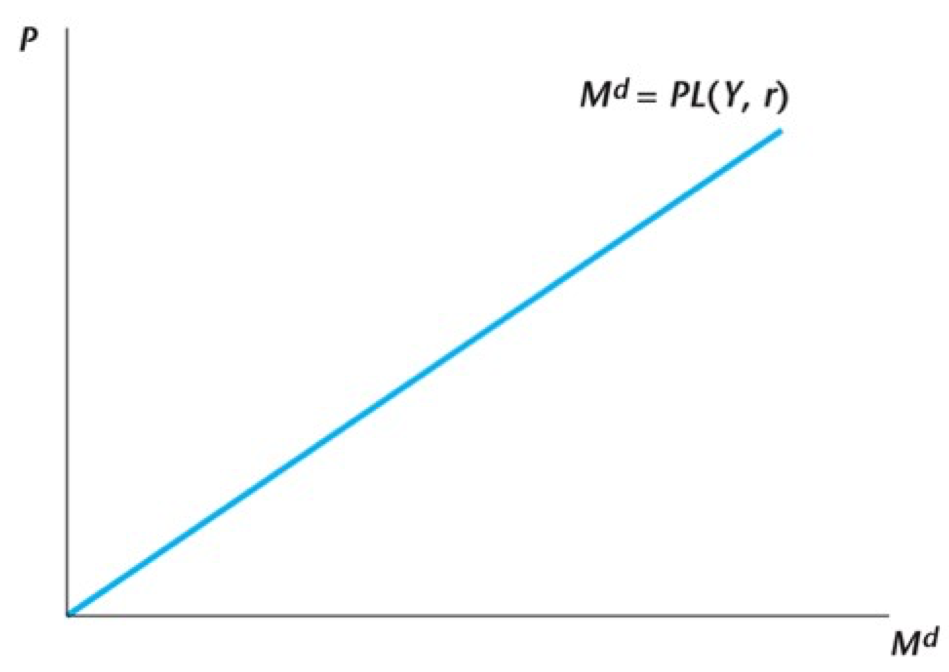
\includegraphics[scale=0.65]{Figures/W_Fig_12pt6.png}
\end{figure}
\end{frame}

\begin{frame}
\frametitle[alignment=center]{Increase in Money Demand}
\begin{figure}
\centering
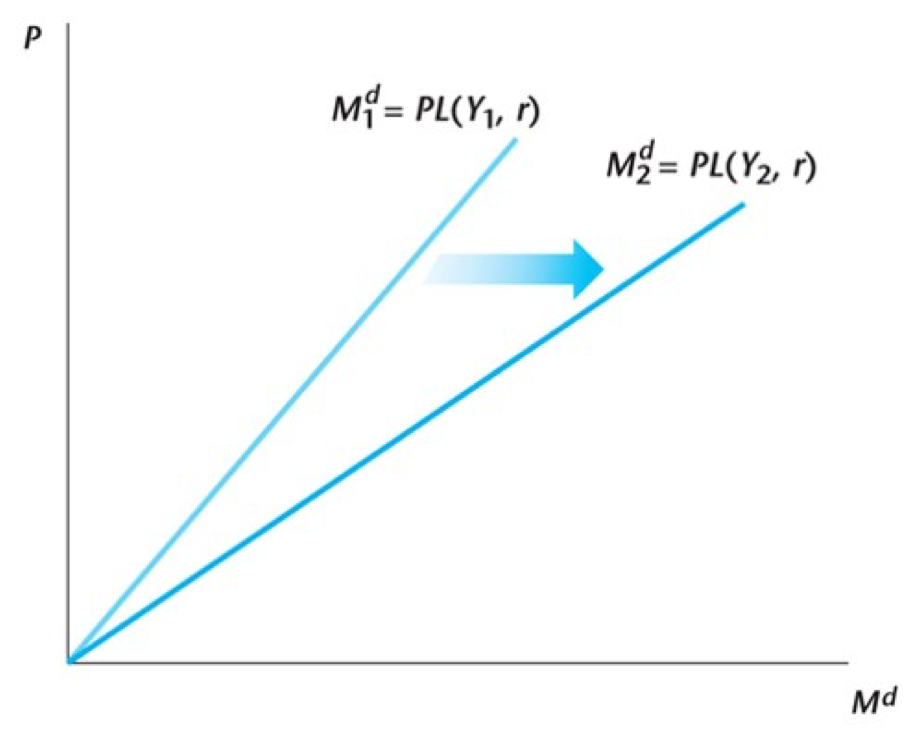
\includegraphics[scale=0.65]{Figures/W_Fig_12pt7.png}
\end{figure}
\end{frame}

\begin{frame}
\frametitle[alignment=center]{Money Supply}
\begin{itemize}
\item We assume government prints money $M$
\bigskip
\item Government budget constraint:
$$PG+(1+R^{-})B^{-}=PT+B+M-M^{-}$$
\item Where $PG$ is nominal expenditure
\item $(1+R^{-})B^{-}$ is retired debt+interest on last period's bonds
\item $PT$ is nominal taxes
\item $B$ is newly-issued bonds
\item $M-M^{-}$ is newly-issued money
\item Now we have money creation and a source for money supply
\item In equilibrium, $M^s=M$, and the price level is determined
\end{itemize}
\end{frame}


\begin{frame}
\frametitle[alignment=center]{Money Supply=Money Demand gives Price Level}
\begin{figure}
\centering
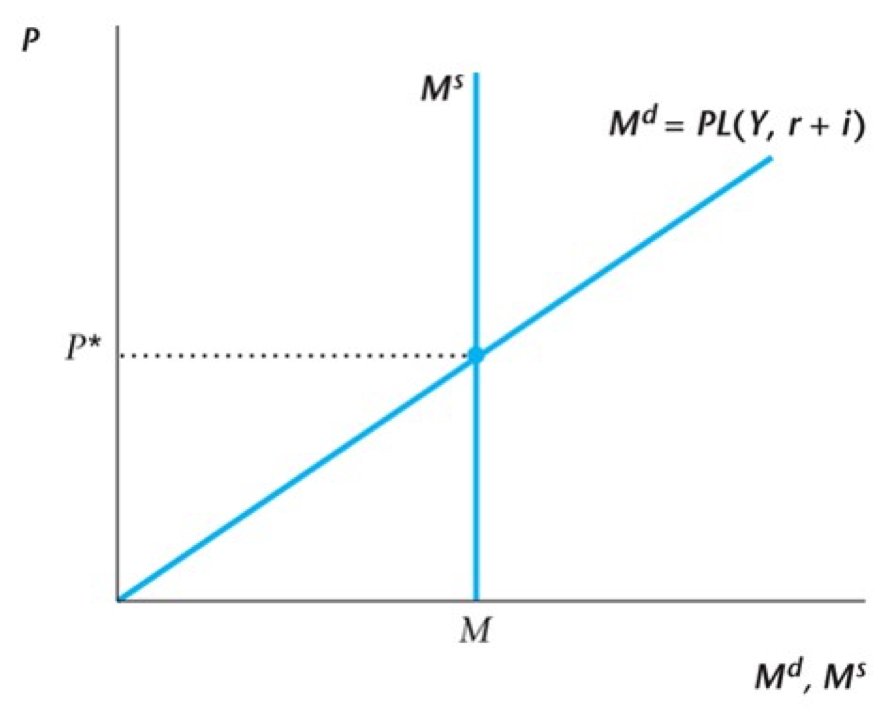
\includegraphics[scale=0.65]{Figures/W_Fig_12pt8.png}
\end{figure}
\end{frame}


\begin{frame}
\frametitle[alignment=center]{Adding in the Price Level to our Intertemporal Model}
\begin{figure}
\centering
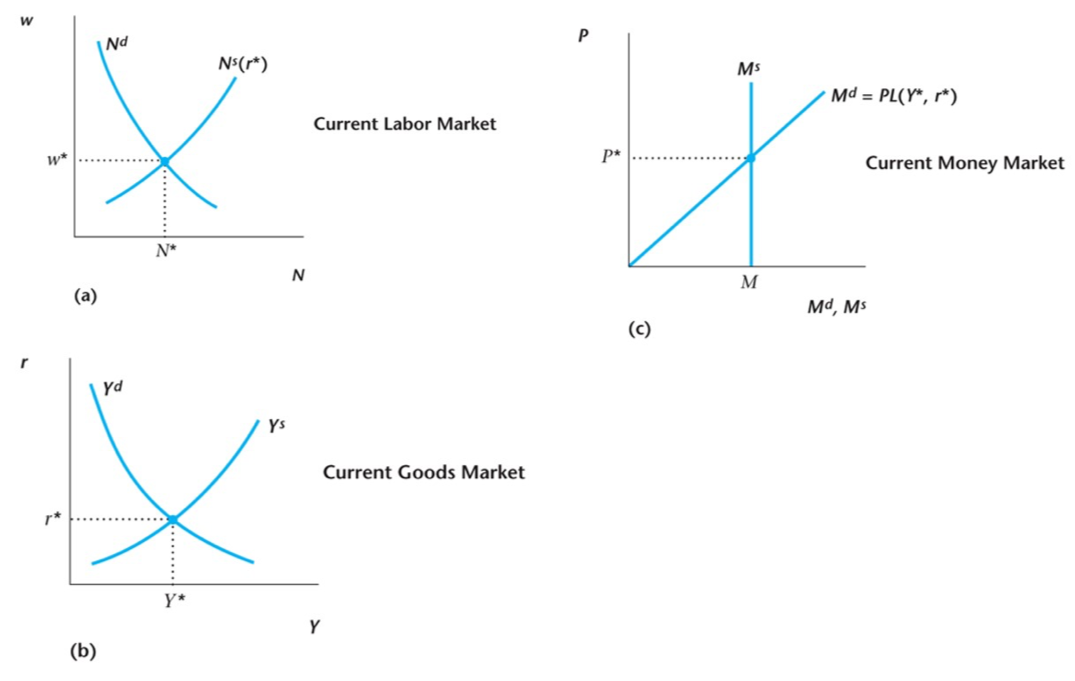
\includegraphics[scale=0.65]{Figures/W_Fig_12pt9.png}
\end{figure}
\end{frame}

\begin{frame}
\frametitle[alignment=center]{Monetary Neutrality}
\begin{itemize}
\item Let's run a one-time experiment of money creation
\end{itemize}
\begin{figure}
\centering
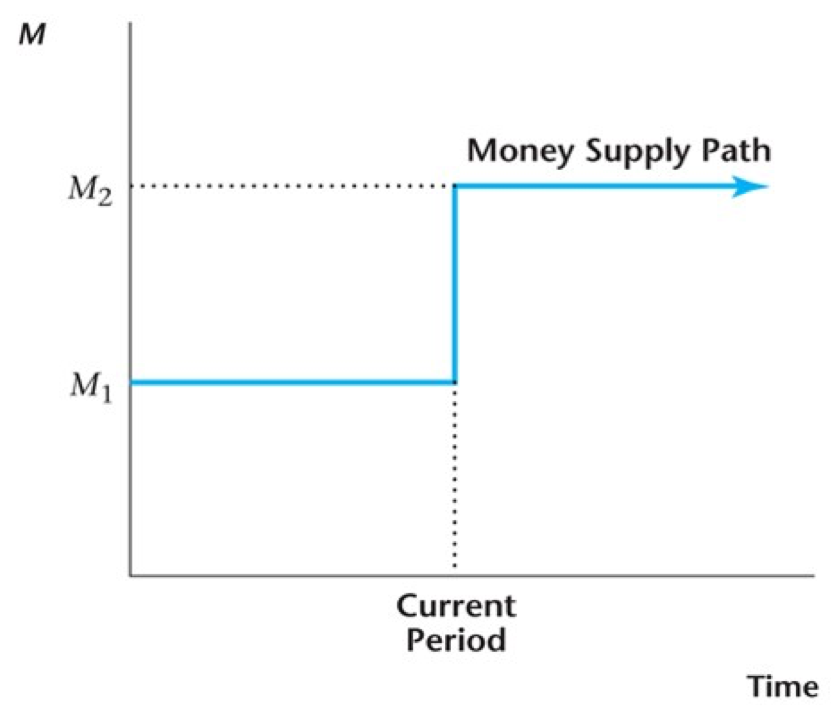
\includegraphics[scale=0.65]{Figures/W_Fig_12pt10.png}
\end{figure}
\end{frame}

\begin{frame}
\frametitle[alignment=center]{Monetary Neutrality}
\begin{figure}
\centering
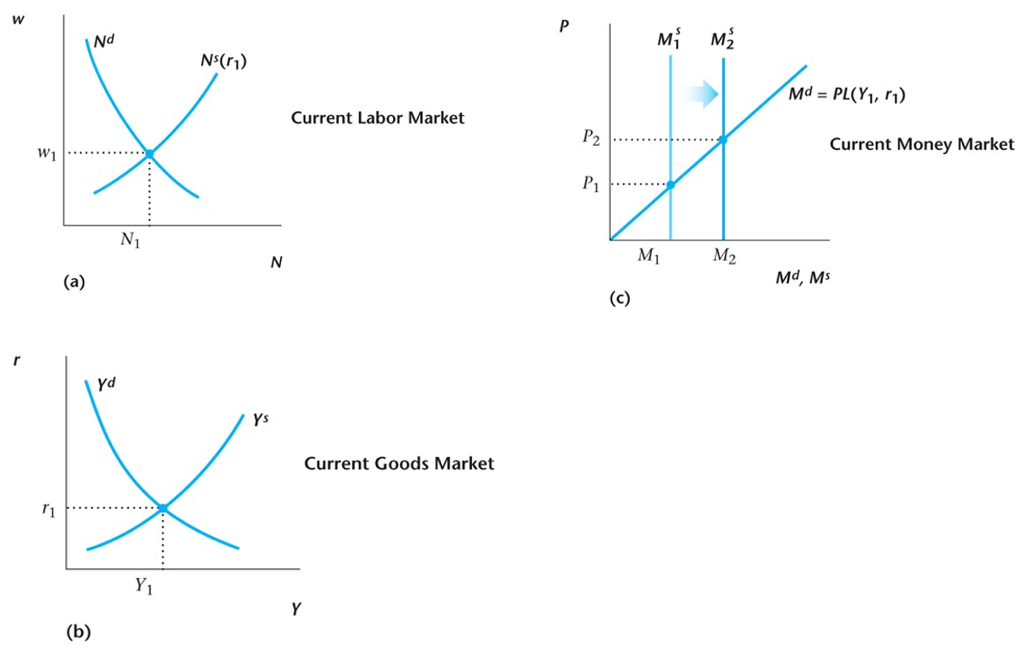
\includegraphics[scale=0.65]{Figures/W_Fig_12pt11.png}
\end{figure}
\end{frame}

\begin{frame}
\frametitle[alignment=center]{Monetary Neutrality}
\begin{itemize}
\item Q: Why is money neutral?
\bigskip
\item A: It doesn't enter into any of the decisions people make, which are based on \emph{real} considerations (real wage, real interest rate)
\end{itemize}
\end{frame}

\begin{frame}
\frametitle[alignment=center]{Shifts in Money Demand}
\begin{itemize}
\item What happens when there's a shift in money demand?  For instance, because the supply of credit becomes tighter
\bigskip
\item Higher demand for money
\bigskip
\item Price level falls
\end{itemize}
\end{frame}

\begin{frame}
\frametitle[alignment=center]{A Shift in the Supply of Credit Card Services}
\begin{figure}
\centering
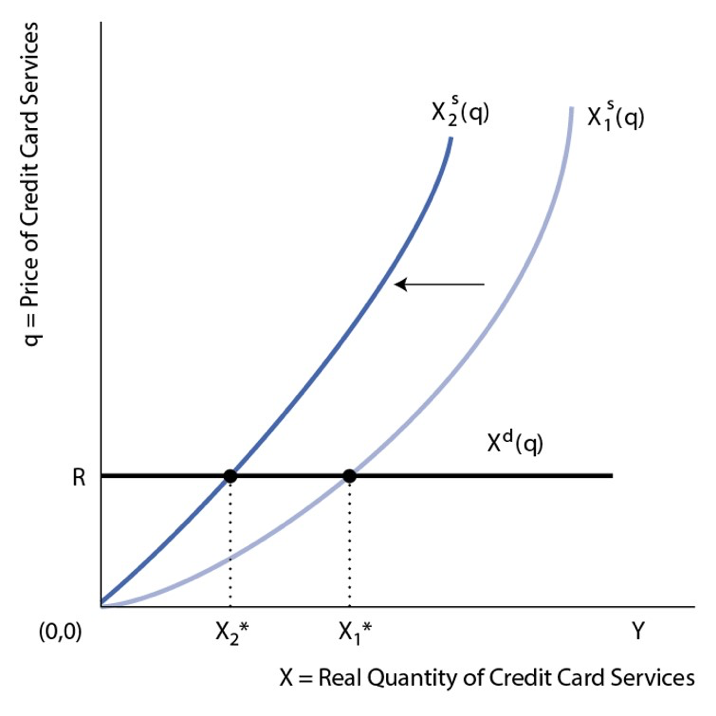
\includegraphics[scale=0.65]{Figures/W_Fig_12pt12.png}
\end{figure}
Higher costs of credit decreases credit use
\end{frame}


\begin{frame}
\frametitle[alignment=center]{Demand for money increases when credit becomes tighter}
\begin{figure}
\centering
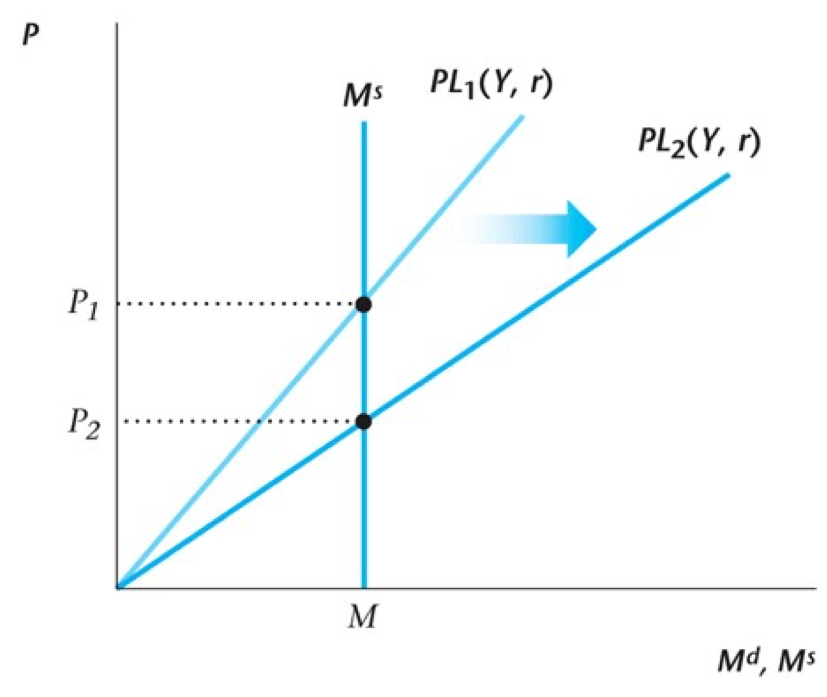
\includegraphics[scale=0.65]{Figures/W_Fig_12pt13.png}
\end{figure}
And increases money use, decreasing price
\end{frame}

\begin{frame}
\frametitle[alignment=center]{Shocks to Money Demand}
\begin{itemize}
\item What might shock the money demand function?
\begin{itemize}
\item New information technologies like ATM's
\bigskip
\item New financial instruments like sweep accounts
\bigskip
\item Changes in government regulations
\bigskip
\item Fear of banks
\bigskip
\item Day-to-day fluctuations (treasuries purchased that day, for instance)
\end{itemize}
\end{itemize}
\end{frame}

\begin{frame}
\frametitle[alignment=center]{Shocks to Money Demand}
\begin{itemize}
\item Okay, so we have a model of price, and how it relates to credit services and money demand and supply
\bigskip
\item It seems like the central bank can control $P$ by controlling $M$, so why did we say it doesn't target/``think about" $M$ very much?
\bigskip
\item Let's look at $L(Y,R)$ in the data
\end{itemize}
\end{frame}


\begin{frame}
\frametitle[alignment=center]{Fitting the Money Demand Function}
\begin{itemize}
\item Let's say we want to match theory and data to answer the question: ``is money demand stable?"
\bigskip
\item Let's try to fit: $L(Y,R)=Ye^{aR}$, where $a$ is a parameter to be estimated
\bigskip
\item Then in equilibrium: $M=PYe^{aR}$, or taking logs:
$$\log\left(\frac{M}{PY}\right)-aR$$
\item Let's graph it!
\end{itemize}
\end{frame}

\begin{frame}
\frametitle[alignment=center]{Money Demand Instability}
\begin{figure}
\centering
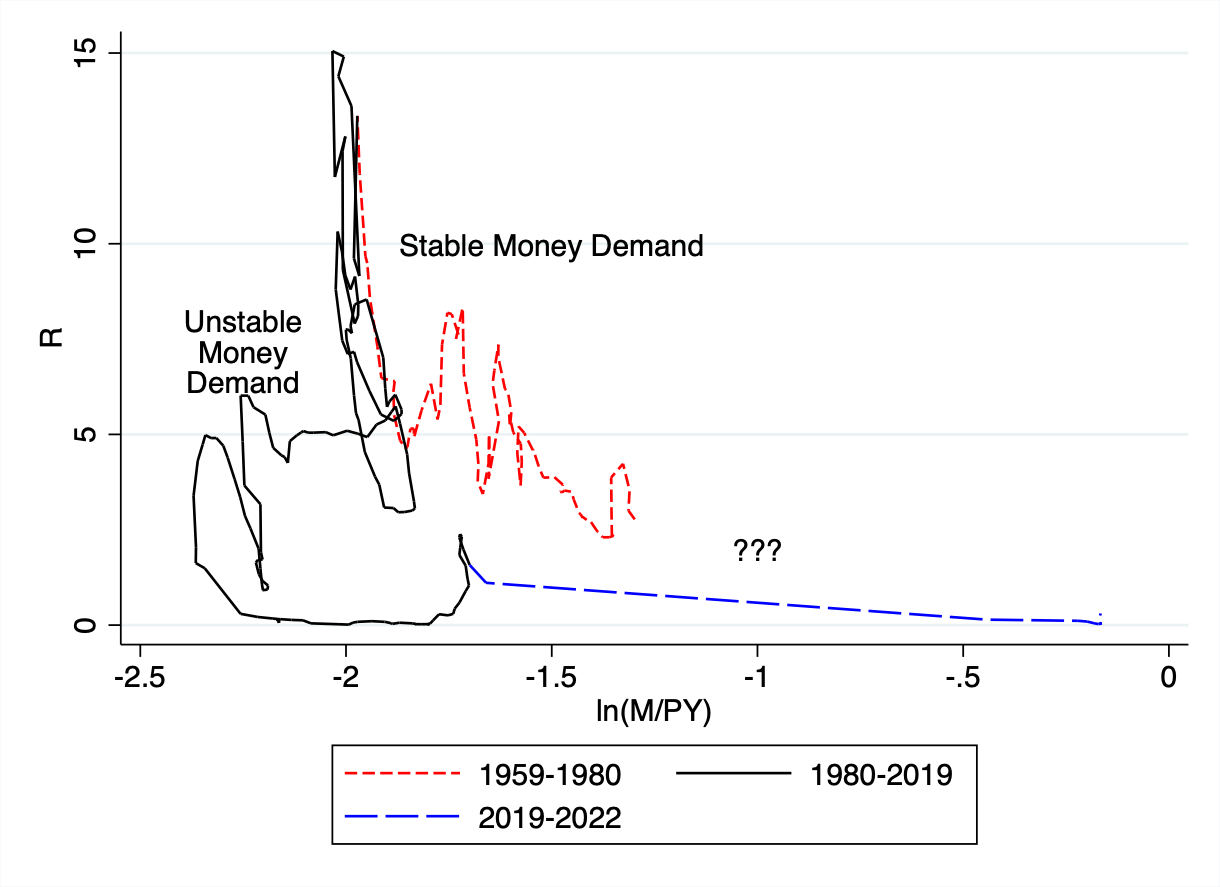
\includegraphics[scale=0.24]{Figures/Fig_12pt14.png}
\end{figure}
Money demand is not very stable post-1980!
\end{frame}


\begin{frame}
\frametitle[alignment=center]{More Modern Monetary Policy}
\begin{itemize}
\item 1970's were dominated by high money supply growth and high inflation
\bigskip
\item ``Monetarists" called for reducing money supply growth to control inflation
\bigskip
\item This occurred, and inflation cooled--but the instability in money demand meant money supply wasn't a fine tool for controlling inflation
\bigskip
\item Now:  eight Federal Open Market Committee Meetings/year, choose the ``federal funds rate", (short-term R)
\bigskip
\item Buy/sell treasuries until market $R$ is target $R$.
\bigskip
\item But, a problem--what if target $R<0$?  ``zero lower bound"
\end{itemize}
\end{frame}

\begin{frame}
\frametitle[alignment=center]{We hit the ``zero lower bound"}
\begin{figure}
\centering
\includegraphics[scale=0.27]{Figures/Fredgraph.png}
\end{figure}
\end{frame}


\begin{frame}
\frametitle[alignment=center]{Zero lower bound}
\begin{itemize}
\item Targeting $R$ worked well for a while
\bigskip
\item But, a problem--what if target $R<0$?  ``zero lower bound"
\bigskip
\item Bank can't force people to accept less than zero--otherwise just hold cash
\bigskip
\item When $R=0$, then bonds and money are the same (both return zero) so Fed can't do anything by switching bonds and cash: open market operations are useless 
\end{itemize}
\end{frame}

\begin{frame}
\frametitle[alignment=center]{Quantitative Easing}
\begin{itemize}
\item What can we do at the zero lower bound?  Short-term B and M are equivalent
\bigskip
\item Could exchange longer-term B for M!
\bigskip
\item This is the heart of ``quantitative easing," purchasing longer-term securities (shifting demand for such assets out) to drive down prices (interest rates)
\end{itemize}
\end{frame}

\begin{frame}
\frametitle[alignment=center]{QE}
\begin{figure}
\centering
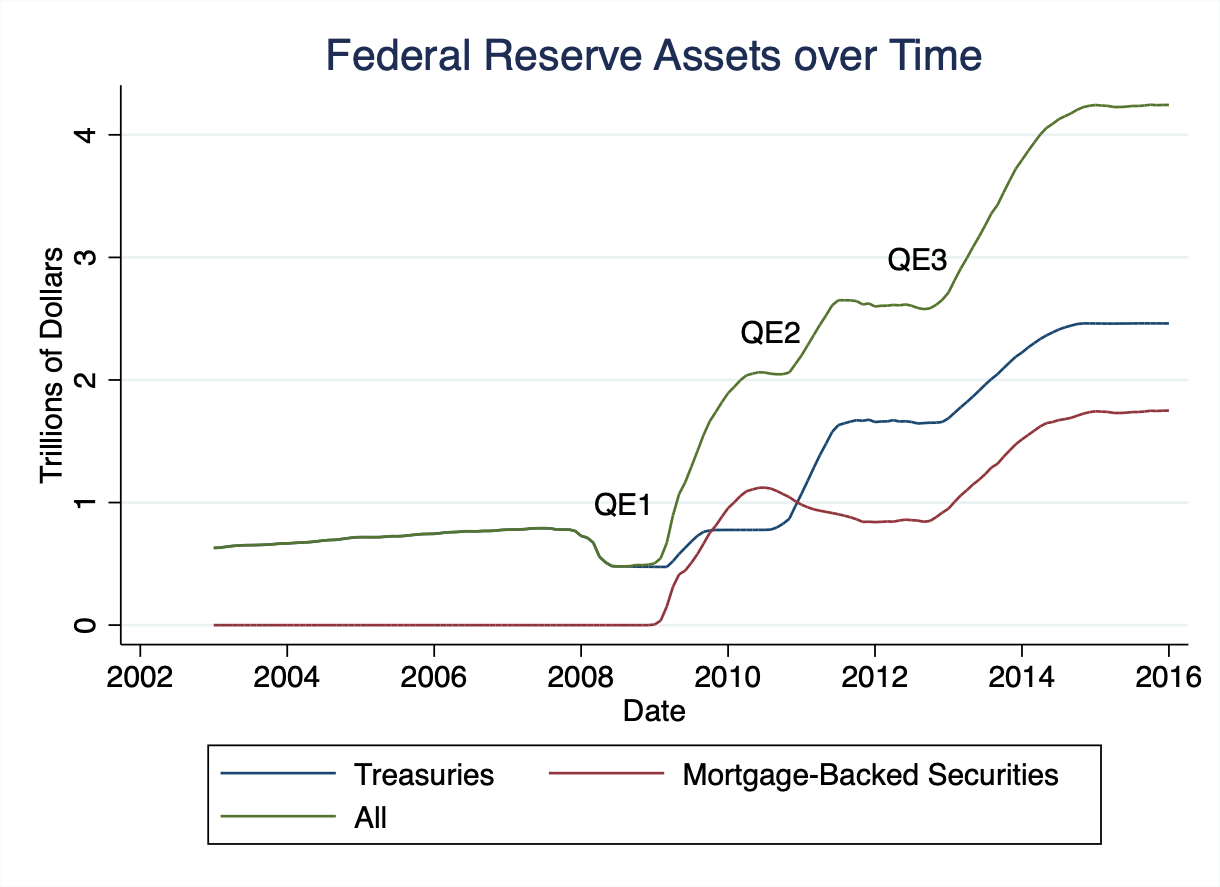
\includegraphics[scale=0.2]{Figures/Fig_12pt16a.png}
\end{figure}
\end{frame}

\begin{frame}
\frametitle[alignment=center]{QE-New!}
\begin{figure}
\centering
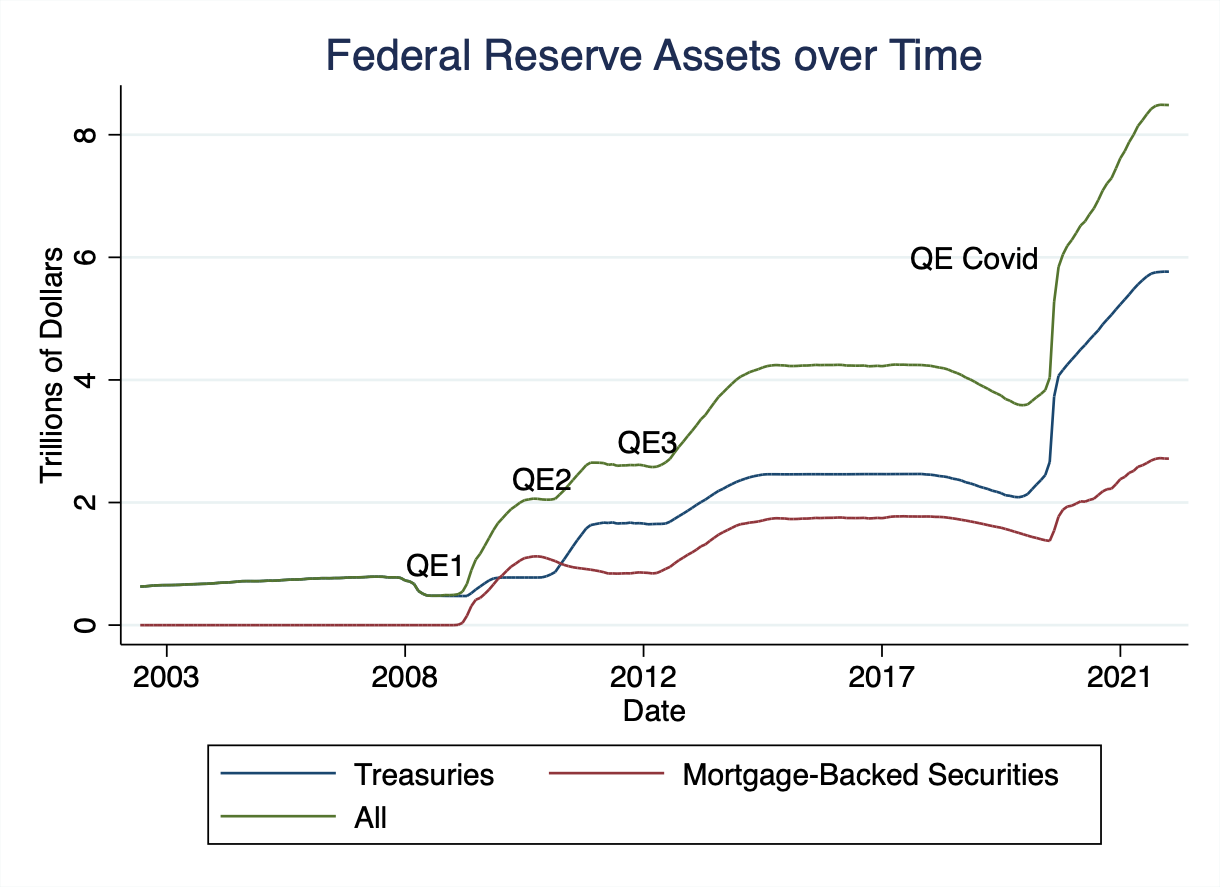
\includegraphics[scale=0.2]{Figures/Fig_12pt16b.png}
\end{figure}
\end{frame}

\begin{frame}
\frametitle[alignment=center]{Summary}
\begin{itemize}
\item Now we have money in our model!
\bigskip
\item But it doesn't do much...monetary neutrality!
\bigskip
\item Evidence monetary neutrality is true!
\bigskip
\item Can analyze the effects of different shifts on the price level
\bigskip
\item Can discuss monetary policy: OMO, QE
\end{itemize}
\end{frame}


\end{document}